\chapter{Troubleshooting and Help}%
\label{cha:troubleshooting_help}

You can report potential problems, bugs, and crashes to the \CGG{} website at:

\begin{center}
	\href{https://www.cinelerra-gg.org/}{https://www.cinelerra-gg.org}
\end{center}

Here you can log the problem into the MantisBT bugtracker, or use the forum Q\&A for help from other users, or email the
problem using the address:{\small \href{mailto:cin@lists.cinelerra-gg.org}{cin@lists.cinelerra-gg.org}} It is usually more
helpful if instead of starting \CGG{} from its application icon, start from a window so that if there are error
messages related to the problem, they can be captured from the screen and emailed or logged. The command to run
from a window is: \texttt{<directory\_path of where you installed cinelerra>/bin/cin} -- for example if
installed in \texttt{/mnt0/build5/cinelerra-5.1}, you would execute the following command to start the program:\\
\texttt{/mnt0/build5/cinelerra-5.1/bin/cin} \\
The problem you are experiencing may be as simple as an error due to the settings in your \texttt{\$HOME/.bcast5} subdirectory so you may want to first rename your current \texttt{.bcast5} in order to start with default settings. By renaming the directory instead of deleting it, you will be able to put it back and not lose all of your preferences.

However, there are some easy things to do to fix errors that may have resulted from media problems,
computer problems, or operational missteps so you can proceed without having to wait for help.  These
are outlined in \ref{cha:when_things_go_wrong} - be sure to read down through
\textit{Common Problems} where some exact error messages are mentioned along with their cause or solution.  Other 
troubleshooting help is included in other sections of this manual for specific features.

\section{What to Include in Problem Reports}%
\label{cha:include_in_problem_reports}
For the best help, if you have a reproducible problem and can provide the following list of materials for analysis, it
is usually possible to figure out what the problem is and how to fix it. It may be a simple usage or setup mistake or
a real bug which a programmer would like to fix rather quickly. Although it is not always necessary to provide this
much information, it eliminates the \textit{try this} or \textit{did you do this?} and a lot of \textit{guessing} rather than heading straight for a solution. \textcolor{red}{Even if you can not provide all of this information, please report the problem in case other users are having the same issue.}

Basically we\textbf{ need to see what you see }with the input, output, and session file. Here is a list of the items that will most likely help to resolve the problem, but all of them will not necessarily be needed.

\begin{itemize}[nosep]
	\item Provide a detailed description of the problem and the last operation performed if you remember it.
	\item Supply a small representative sample of the original input that exhibits the issue.
	\item If possible, also provide the rendered output, again using that representative sample.
	\item Save a session file used with that same sample which will contain a lot of setup parameters; the best method to do this is to use the \texttt{File $\rightarrow$ Export Project}$\dots$ with the Copy option. That way all of the files will be in 1 location and easily loaded onto any other computer.
	\item To make sure that the same rendering setup is used, it may be necessary to send an additional session file at the definition point just before rendering starts.
	\item Include the Operating System name and version number and version of Cin that you are running. You can find the date and time \textit{built} in the \texttt{Settings $\rightarrow$ Preferences, About} tab, bottom left corner.
\end{itemize} 

It is better to upload any files to a drop site as some of them can be quite large.

\textbf{How to create a session file:} \quad from the menubar pulldown \texttt{File $\rightarrow $ Save\_as}{\dots} \quad and choose a filename, for example \texttt{/tmp/beforerender.xml} Do this after you have the situation setup so can see values in use. As just stated, \textit{Export Project} option provides the most inclusive session information, but size could make it very large and cumbersome to upload or download.

\textbf{How to create a representative small sample:}

\begin{enumerate}[nosep]
	\item open the input media, set up the scenario as you normally would to start the project render;
	\item select 5-15 seconds of media using the edit mode left mouse button drag highlighting on the timeline;
	\item start the render dialog (Shift-R), set the filename path, and set \textit{Render range} to \textit{Selection};
	\item recommended \textit{Insertion strategy} is \textit{Replace current project}; then press the checkmark OK. The result will \textit{load replace} the current project for you to review to ensure the error still occurs. If this small sample does not create the error, try a different section or upload the entire input media.
\end{enumerate}


\section{Crash Dumps for Analysis}%
\label{cha:crash_dumps_analysis}
If you get a SEGV crash and can explain what steps you took, a \texttt{/tmp/cinelerra\_<pid> .dmp} file is
very useful for analysis. You can also use Ctrl-c in the controlling window to force an INTR signal interrupt when
you think the program is hung up. You can only perform one Ctrl-c as the second Ctrl-c quits out of the program. It
is best to upload the \texttt{.dmp}, input files and other files to datafilehost or similar temporary site as they may be quite large. The \texttt{.dmp} filename looks like \texttt{/tmp/cinelerra\_<pid> .dmp} Log a bug report or email all
helpful information on the crash, location of uploaded files, and list of setup steps that illustrate the problem to
{\small \href{mailto:cin@lists.cinelerra-gg.org}{cin@lists.cinelerra-gg.org}}

\begin{enumerate}[nosep]
	\item Use the latest version of \CGG{} as you want to make sure the problem has not been fixed.
	\item Be sure \textit{gdb} is installed (usually installed but if not, it is easy to do so).
    \item Run as root if at all possible (this enables using gdb to create a full \texttt{/tmp/cinelerra* .dmp} file).
    \item Be sure \texttt{Settings $\rightarrow$ Preferences $\rightarrow$ Interface $\rightarrow$ trap SEGV} and \texttt{trap INTR} are checked.
	\item Invoke the error. This should create the file \texttt{/tmp/cinelerra-<pid>.dmp}
\end{enumerate}
\medskip

For those who can not run as root or can not create the problem while running as root, another method to create a dump
is available. Here are the steps to do so -- you should also have gdb installed.
\medskip

\begin{enumerate}[nosep]
	\item Temporarily login as root and key in:\\
	\texttt{echo 0 > /proc/sys/kernel/yama/ptrace\_scope} \\
	This opens up \textit{ptrace}, used by gdb (the debugger). You will want to reverse this when done.
	\item Run \CGG{} as an ordinary user from a window using the command line and try to create the problem. If the program crashes, this should produce a file named \texttt{/tmp/cinelerra*.dmp} where * is a number. The dump usually takes about 30 seconds or so to complete after the failure invokes the crash handler, so be patient. 
	\item Email the output that shows in the window from where you started up \CGG{} and upload or directly email the \texttt{/tmp/cinelerra*.dmp} file (this file may be too large for the Mailing List).
	\item After you are finished creating/testing the problem, reverse the previous setting while logged in as root by keying in:\\
	\texttt{echo 1 > /proc/sys/kernel/yama/ptrace\_scope}
\end{enumerate}

\textcolor{red}{Even if you are not logged in as root or have ptrace enabled, if you
have a .dmp file and know what the last thing you did is, please provide the .dmp file for analysis.} There is a low
probability that the dump will prove useful, but if the problem can be recreated it can usually be fixed!

\section{When things go wrong}%
\label{cha:when_things_go_wrong}
Sometimes things go wrong and there are some ways to continue your work without much trouble. Below is a list of items
to try before abandoning your session.

\begin{enumerate}
	\item If you suddenly get errors or hangs on media or strange looking tracks, you might want to rebuild indexes. You can do this in the Resources window with a right mouse click on the media to get a pulldown with the \textit{Rebuild index} option. For an easy way to rebuild for all of your media use \texttt{Settings $\rightarrow$ Preferences, Interface} tab, Index Files section, \textit{Delete existing indexes}. Over time, as you
load media, the indexes will automatically be recreated so each load takes a little longer, but this quite often
is all that is needed to repair a media problem.
	\item On an older computer, if you are playing media and it can not keep up, you can turn off \textit{Play every frame} in the \textit{Video Out} tab of \texttt{Settings $\rightarrow$ Preferences, Playback} tab. You will then see the video jump as it skips frames in order to stay caught up.
	\item The \textit{Cache size} can be lowered to 1048 if playback seems choppy or if you have problems with lv2 plugins, or you can increase the \textit{Cache size} for better flow. This can be changed in \texttt{Settings $\rightarrow$ Preferences, Performance} tab.
	\item After saving your session and settings and exiting \CGG{}, you might want to rename your current \texttt{\$HOME/.bcast5} directory and start with the default setup. This will eliminate your settings as the potential cause of a problem; however, all of your preferences will be lost until you go back to your original \texttt{.bcast5}.
        \item You can also temporarily rename just \CGG{}\_rc in your \$HOME/.bcast5 directory, so
that a new file with the original name will be created with original defaults.  You will lose your preferences,
but it is just for testing and you can move back the renamed \CGG{}\_rc over the new one if that is not the
cause of the problem.  Be sure to stop and restart \CGG{} whenever you rename this file.
	\item Some media has only a single keyframe at the beginning of the file so that moving anywhere on the timeline results in just a black image in the compositor. \CGG{} needs more keyframes to determine position. You can temporarily use \texttt{Settings $\rightarrow$ Proxy} to $\frac{1}{2}$ size to put in keyframes. How to use Proxy is explained in \href{sec:proxy_settings}{Proxy settings and Transcode}.
        \item If you have enabled an \textit{Automation Curve} such as Fade or Speed on your track but it
does not show, it could simply be because the range minimum and maximum are incorrectly set in the zoom bar.
Set them to more reasonable values until you see the lines appear. Just as a reminder, the zoom bar is on the
bottom of the main window (figure~\ref{fig:automation}). 
 	\item If the rate at which frames are captured during Recording is much lower than the framerate of the source, the video will accumulate in the recording buffers over time and the audio and video will become out of sync. Decrease the number of frames to buffer in the device in \texttt{Settings $\rightarrow $ Preferences, Recording} tab so that the excess frames are dropped instead of buffered.
	\item If loading files locks up, this might be because \CGG{} is building picons/vicons for the Resources window. If you load a large number of images it needs to decompress every single image to build a picon/vicon. Go into \texttt{Settings $\rightarrow$ Preferences, Appearance} tab and disable \textit{Use thumbnails in resource window} to skip this process. Keep in mind though, that it only has to create these thumbnails the first time a new piece of media is loaded or the values are changed.
	\item For an older computer with less CPU power, in \texttt{Settings $\rightarrow$ Preferences, Appearance} tab, be sure that \textit{Autocolor assets }is disabled; set \textit{View thumbnail size} \& \textit{Vicon quality}\& \textit{Vicon color mode} to lower values or switch to \textit{No Play} instead of \textit{Full Play} in the Resources window (this is to the right of the word \textit{Visibility} in the left hand side of that window). You will then have more CPU and more memory available to do actual editing.
\end{enumerate}

\textbf{Some Helpful User Readable Text Dumps}

On the File pulldown, there is a \textit{Dumps} option with a submenu of dump EDL, Plugins, Assets, and Undo. In all cases, you will have to have started \CGG{} from a window instead of from an application icon and
the text results will be shown in that window.

\begin{itemize}[nosep]
\item \textit{Dump EDL} will display your current EDL state on the screen in the window from where you started Cin. This can be useful to see information concerning a specific edit or a file path.
\item \textit{Dump Plugins} will show the names of the currently loaded plugins.
\item \textit{Dump Assets} displays the media assets that you have loaded and various pertinent details on each, such as samplerate, width, and height.
\item \textit{Dump Undo }will dump the last 32 edits on the undo stack exactly as kept, which can be useful if you are looking to see how far back in the undo to go to get to a specific spot.
\end{itemize}

\textbf{Common Problems}

Some messages you may see in the startup window may or may not be errors. Some examples are:
\bigskip

\textit{FFMPEG::open\_decoder: some stream times estimated:} \quad \texttt{/your directory/filename}

This is not a problem. Basically, when you open a file if a stream has a known duration, there is no message. If the duration is unknown, it is estimated by using the File Size and Bitrate to estimate the duration. This may just indicate that the stream number \CGG{} uses versus ffmpeg may be counted differently.
\bigskip

\textit{AudioALSA::write\_buffer err -32(Broken pipe) at sample \#}

This indicates that there is something wrong with the audio. Some reasons for this are:
\begin{itemize}[nosep]
	\item You simply stopped playing in \CGG{} while the audio is in progress.
	\item Running on a computer where there is no sound card.
	\item Incorrect setup of the audio parameters in the \texttt{Settings $\rightarrow$ Preferences, Playback} tab.
	\item Your sound system is already in use by another program, like when playing \textit{tunes} outside Cin.
\end{itemize}
\bigskip

\textit{Playback does not keep up so you hear the audio ahead of the video.}

When this occurs, it most likely means that there is not enough CPU power to keep up. You can go into \texttt{Settings $\rightarrow$ Preferences, Playback} tab and uncheck \textit{Play every frame}. Not playing every frame means that as it plays, if it can not keep up with doing all it has to do to change the frame into a vframe and then draw it, the program just notes that it is falling behind so skips frames to catch back up. This does not affect rendering. A different solution is to use Background Rendering as described in \href{sec:background_rendering}{Rendering}.
\bigskip

\textit{\CGG{} will not start and produces error message on the startup window.}

There can be various reasons that \CGG{} does not come up. Some of the recent reasons are listed here. Please notify the {\small \href{http://www.cinelerra-gg.org/}{www.cinelerra-gg.org}} website when you have any unknown startup issues.
\medskip

\begin{itemize}[nosep]
	\item Cin doesn't come up in Debian with compiz window manager running. Workaround is to use a different window manager or bring up cin first and then compiz. There is also a report that Compiz leads to single frame problems after a certain amount of time in the case where you switch to fullscreen mode and than back to normal node -- cin stops working and so you will have to restart cin.
	\item When a library goes from one version to a later version, sometimes a pre-built Cin binary will fail because it was created at a different version than the one the user has on their computer. This seems to happen more frequently on Arch distros because Arch has continuous releases and is usually kept up to date. An example of the error message you might see in your startup window would be:\\
	\texttt{cin: error while loading shared libraries: libvpx.so.5: \\
	cannot open shared object file: No such file}
\end{itemize}
\medskip

You can usually install the required library to fix the problem. A temporary fix may be to create a symlink but this must be done with extreme caution as it may create an unstable condition. A better workaround is to use a tarball to install the software instead of the package build until the libraries are in sync between the build and your Operating System install.
\bigskip

\textit{ Loading a very large number of media files, for example 500 clips, crashes \CGG{} with messages similar to the following that are displayed in the window from where you started Cin:}

\begin{lstlisting}[numbers=none,xleftmargin=10mm]

   BC_DisplayInfo::init_window: cannot open display "".
   BC_DisplayInfo::init_window: cannot connect to X server.
   unjoined tids / owner 42
     00007feb27fff700 / 00007feb8f496700 9MainError
     00007feb267fc700 / 00007feb7affd700 18FFMPEGScanProgress
     ... 

\end{lstlisting}

This usually indicates that you are out of Operating System file descriptors.  You can increase the amount easily with the following command line:  \texttt{ulimit -n 4096}   where 4096 is a size suggestion but can be increased.  You can include this command line in your \texttt{.bashrc} or \texttt{.profile} file for the user login which gets run every time you login, or modify the Operating System limit for everyone in the system file, which for Fedora is \texttt{/etc/security/limits.conf}.  Alternatively, you can reduce the number of file descriptors needed by going into \texttt{Settings $\rightarrow$ Preferences, Appearance} tab and unchecking the flag \textit{use thumbnails in resource window}.

\bigskip
\textit{Masking Feather is not working and produces error messages on the startup window similar to:}

\begin{lstlisting}[numbers=none,xleftmargin=10mm]
0:1(10): error: GLSL 4.30 is not supported. Supported versions are: 1.10, 1.20, 1.30, 1.40, 1.00 ES, and 3.00 ES
Playback3D::print_error:
#version 430 // vertex shader
in vec3 in_pos;
void main000() \{
gl_Position = vec4(in_pos-vec3(0.5,0.5,0.), .5);
}
void main() \{
main000();
}
\end{lstlisting}

In the mask window, check the box \textit{Disable OpenGL masking} to use software instead of OpenGL.

\section{Menu Bar Shell Commands}%
\label{menu_bar_shell_commands}

In order to provide some types of help, the Menu Bar Shell Commands are available for customization purposes. In the
main window on the top line containing the File, Edit, {\dots} Window pulldown menus, all the way to the right hand
side is the \textit{shell cmds} icon. You might see a small gold-color bordered box with the $>\_.\_$ inside
and if you mouse over it, the tooltip says \textit{shell cmds}. This is a configurable popup which gives you the ability to
see a table of Shortcuts in html format, refer to the reference manual or execute a pre-defined script to perform a
specific task, such as some type of post processing which you plan on performing on a repeat basis. Unless redirected
elsewhere, the output from executing any script-type commands will be displayed in the window from where you started
\CGG{}.

The Shell Cmds popup menu items are configured in:

\texttt{Settings $\rightarrow$ Preferences $\rightarrow$ Interface $\rightarrow$ Shell Commands}

This runs a dialog that lets you Add/Del/Edit the scripts in the main menu popup. \ Possible options are:\newline

\begin{enumerate}
	\item \textit{Add} a new menu item/script:
	\begin{itemize}[noitemsep]
		\item click on the \textit{Add} button
		\item in the Label box, change the word \textit{new} to the desired menu label (for example: Graphics Editor)
		\item in the Commands box, type the command lines to be included in the script (for example: gimp)
		\item click the green checkmark for OK in the Commands window
		\item click the green checkmark for OK in the Shell window
		\item click on OK or Apply in the Preferences window
	\end{itemize}
	\item \textit{Del} to delete an existing menu item
	\begin{itemize}[noitemsep]
		\item select to highlight an entry in the \CGG{}: Shell listbox
		\item click on the \textit{Del }button
		\item click the green checkmark for OK in the Shell window
		\item click on OK or Apply in the Preferences window (the entry is now deleted)
	\end{itemize}
	\item \textit{Edit} an existing menu item:
	\begin{itemize}[noitemsep]
		\item select to highlight an entry in the \CGG{}: Shell listbox
		\item click on the \textit{Edit} button (the Commands window appears)
		\item set the label and/or commands to the new desired values
		\item click on the green checkmark for OK in the Commands window
		\item click on the green checkmark for OK in the Shell window
		\item click on OK or Apply in the Preferences window
	\end{itemize} 
\end{enumerate}
	
Next time you click on the \textit{shell cmds} icon, you will have the changes you made in effect.

Both the \textit{Add} and \textit{Edit} options have checkboxes in the Commands window for the following:

\begin{itemize}[nosep]
	\item \textit{OnExit notify} \quad  choose Always, Never, or On error to get a popup window notify
	\item run \texttt{path/script.sh + argvs} \quad to run a particular script with argvs (\$1, \$2,{\dots} arguments)
\end{itemize}


When modifications to the Shell Cmds are included in a new \CGG{} release, they are not added to your Preferences file automatically unless you create a new one. But if you have added no custom scripts, you can update your currently existing \texttt{\$HOME/.bcast5/ \CGG{}\_rc} file to delete the lines that are all grouped together that begin with the letters: \texttt{SHBTN} (the entire line -- these are the \textbf{SH}ell \textbf{B}u\textbf{T}to\textbf{N}s). \ You should first Quit out of \CGG{}, edit the file, and then when you restart \CGG{}, it will create the new default buttons in that same file.

There are 2 specific \CGG{} file names that have unique characteristics that allow for usage from a user-defined
script. The first one is an environment variable, \texttt{CIN\_RENDER} which is used in the \textit{RenderMux} shell command that is already setup. It contains the complete path and filename of the file in your session that you selected as \textit{Select a file to render to} when you ran a Render operation.

The second one concerns usage of the Resource window assets to use as argvs in shell scripts. The added command line
can ONLY be a script. Then if your script refers to \$1, \$2 and \$3 and you highlight 3 files in the Media folder,
their full path name will be used as the argvs to your script. For example, if you added a shell commands script
\texttt{/workspace/script.sh} that contains the following lines:

\begin{lstlisting}[numbers=none,xleftmargin=10mm]
cp ``\$1'' /tmp/temporary_copy
cp ``\$2'' /tmp/new_copy
cp ``\$3'' /tmp/file_to_upload
\end{lstlisting}

and you highlight 3 files in the Resources window called\textit{ ABC.mp4}, \textit{123.mp4}, and \textit{Final.mp4} and execute your added script from the Shell Cmds icon, you will be copying those 3 highlighted files to the new names on \texttt{/tmp}.

There are some Help features currently included in the Shell Cmds menu. Those available are:

\begin{enumerate}
	\item \textit{Current Manual} in PDF format from cinelerra-gg.org or automatically downloaded.
	\item \textit{Setting Shell Commands} \textit{how to} which explains how to configure your own commands.
	\item \textit{Shortcuts} html file for easily looking up a particular shortcut.
	\item \textit{RenderMux} shell script to use ffmpeg concatenate to copy files such as \textit{look.mp4001}, \textit{look.mp4002}, \textit{look.mp4005}{\dots} that were rendered using \textit{Create new file at each label} or with the Render Farm.
\end{enumerate}
\clearpage

\begin{figure}[h!]
	\centering
	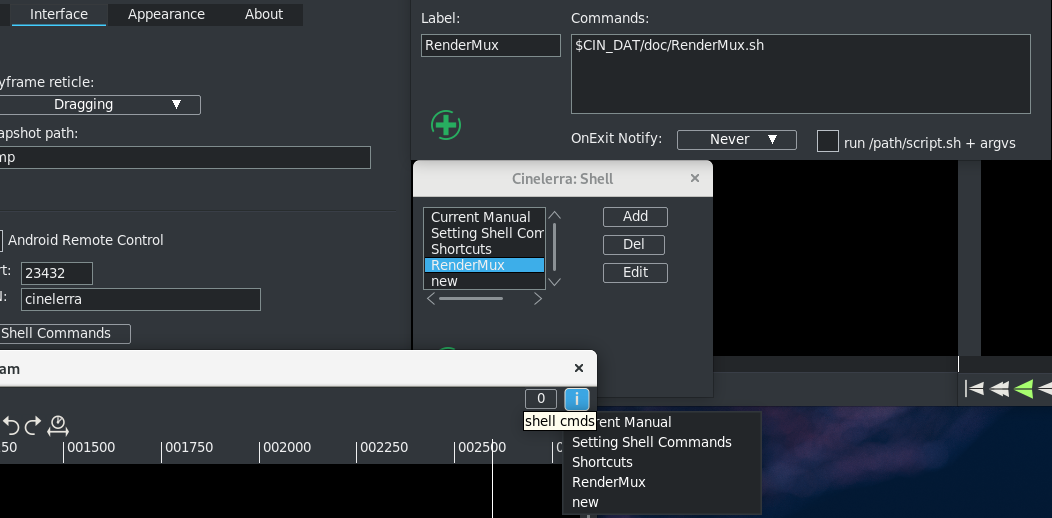
\includegraphics[width=1.0\linewidth]{trouble-img001.png} 
	\caption{Some windows used to manipulate Shell Commands scripts}
	\label{fig:shell_script_manupulation}
\end{figure}

\section{\CGG{} Command Line -h}%
\label{cha:cinelerra_command_line_-h}

To see the command line parameters available to use with \CGG{}, key in:

\qquad \texttt{<your \CGG{} directory path>/bin/cin -h}

What will be shown in the window where this line was entered is:

Usage:

\texttt{./cin [-f] [-c configuration] [-d port] [-n nice] [-r batch file] [filenames]}

-d = Run in the background as renderfarm client.  The port (400) is optional.\\
-f = Run in the foreground as renderfarm client. Substitute for -d.\\
-n = Nice value if running as renderfarm client. (19)\\
-c = Configuration file to use instead of /root/.bcast5/Cinelerra\_rc.\\
-r = batch render the contents of the batch file (/root/.bcast5/batchrender.rc) with no gui. batch file is optional.\\
-S = do not reload perpetual session\\
-x = reload from backup\\
filenames = files to load

